\subsection{Surriscaldamento e coibentazione}
L'apparato per la rivelazione dei RC è molto sensibile alla temperatura, e in particolare questa ne influenza l'efficienza. Salendo in quota, è noto che la temperatura vari nel range $-56^{\circ}\text{C} \div 15^{\circ}\text{C}$. Per minimizzare tale variazione si è deciso di coibentare l'apparato con una struttura in polistirolo.

L'elettronica che si vuole utilizzare può facilmente surriscaldarsi (in particolare la FPGA), e ciò può comportare un effetto non controllabile sulla strumentazione. Per minimizzare questo effetto si è pensato di separare fisicamente l'elettronica dall'apparato rivelatore. Inoltre, la strumentazione stessa potrebbe subire malfunzionamenti a causa dell'elevata temperatura: è in corso una valutazione sulla possibilità di inserire delle strips di rame che permettano di dissipare il calore all'esterno dell'elettronica.
% (uno scatch di questa soluzione è illsutrata in Figura \ref{surriscaldamento}).

%\begin{figure}
%    \centering
%    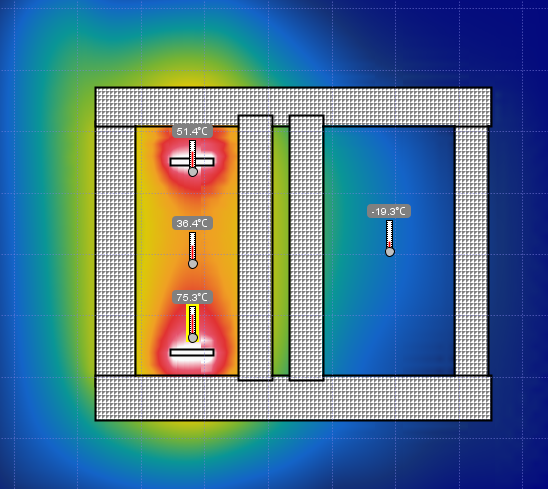
\includegraphics[width=0.3\textwidth]{surriscaldamento.png}
%    \caption{Simulazione \textit{Energy2D}\citep{surriscaldamento}: a sinistra due sorgenti a $80^{\circ}$ con isolamento in polistirolo; a destra uno spazio vuoto in cui allocare l'apparato rivelatore.}
%\end{figure}